\renewcommand{\theequation}{\theenumi}
\begin{enumerate}[label=\arabic*.,ref=\thesubsection.\theenumi]
\numberwithin{equation}{enumi}
\item No of the total students participating the survey=
200
\\
students like the statics = 135
\\
P(A) = probability of student likes the statics
\begin{align}
P\left(A\right) &= \frac{135}{200}
\\
&= 0.675
\end{align}
\\
\item No of students do not like the statics = 65
\\
P(B) = probability of student does not like the statics
\begin{align}
P\left(B\right) &= \frac{65}{200}
&= 0.325
\end{align} 
codes for the above equation can be get from here
\begin{lstlisting}
codes/prob/prob6.py
\end{lstlisting}
\begin{figure}[!ht]
	\centering
	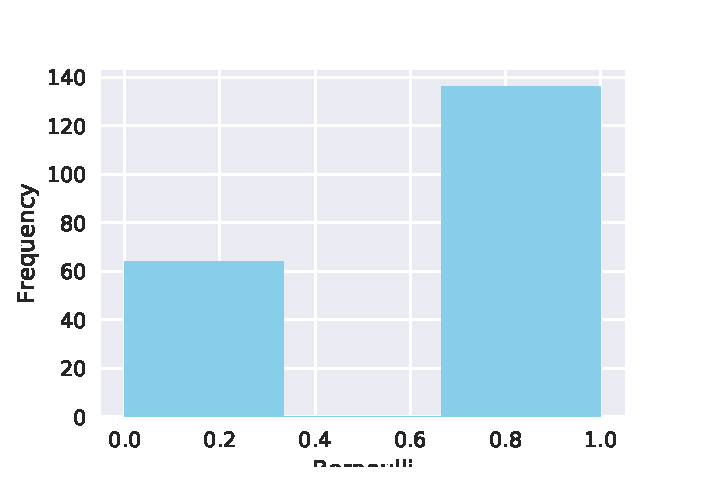
\includegraphics[width=\columnwidth]{./figures/prob/prob6.eps}
	\caption{bernouli distribution of students liking statics }
	\label{fig:bt5}
	\begin{lstlisting}
	figs/prob/prob6.py
	\end{lstlisting}
\end{figure}
\end{enumerate}